\subsection{SOAC: scan}

Second-order Array Combinator (SOAC):\textcolor{red}{\textit{\textbf{scan}}} 是所有的循环神经网络(recurrent neural networks)背后的核心并行pattern。接口和语义如下:

\begin{equation*}
    \begin{aligned}
        \textbf{scan} &::(\alpha, \beta \rightarrow \alpha) \rightarrow \alpha \rightarrow[\beta]^d_n \rightarrow [\alpha]_n^d \\
        \mathbf{scan} \ \oplus \ \textit{xs} &= [x_0,\ x_0 \oplus x_1, \dotsb,\ x_0 \oplus x_1 \dotsb \oplus x_n ] \\
        \mathbf{scanl} \ \oplus \ I \ \textit{xs} &= \left[
            I \oplus x_0,\  ((I \oplus x_0) \oplus x_1), \ \dotsb,
            \ (((I \oplus x_0)\oplus x_1)\dotsb \oplus x_{n-1})
        \right] \\
        \mathbf{scanr} \ \oplus \ I \ \textit{xs} &= \left[
            (x_0 \oplus (x_{n-2} \oplus (x_{n-1} \oplus I)))
            ,\ \dotsb, \ (x_{n-2} \oplus (x_{n-1} \oplus I)),
            \ x_{n-1} \oplus I \right] \\
    \end{aligned}
\end{equation*}


% If $\oplus$ is associative, scan can be executed in parallel\cite{DBLP:journals/tc/Blelloch89}.
% If $\oplus$ is left associative, scanl is used. If $\oplus$ is right associative, scanr is used. The first operand of $\oplus$ carries a data dependence with a distance of 1\cite{DBLP:journals/tpds/WolfL91}.

% \subsection{RNN}

% As shown in Figure \ref{scan-step}, in one computational step, a cell processing unit $\otimes$ produces a new token $y$ by aggregating a token $x$ from a token stream $xs$ with another token $y'$ created in the previous computational step.

% \begin{figure}[h]
%     \centering
%     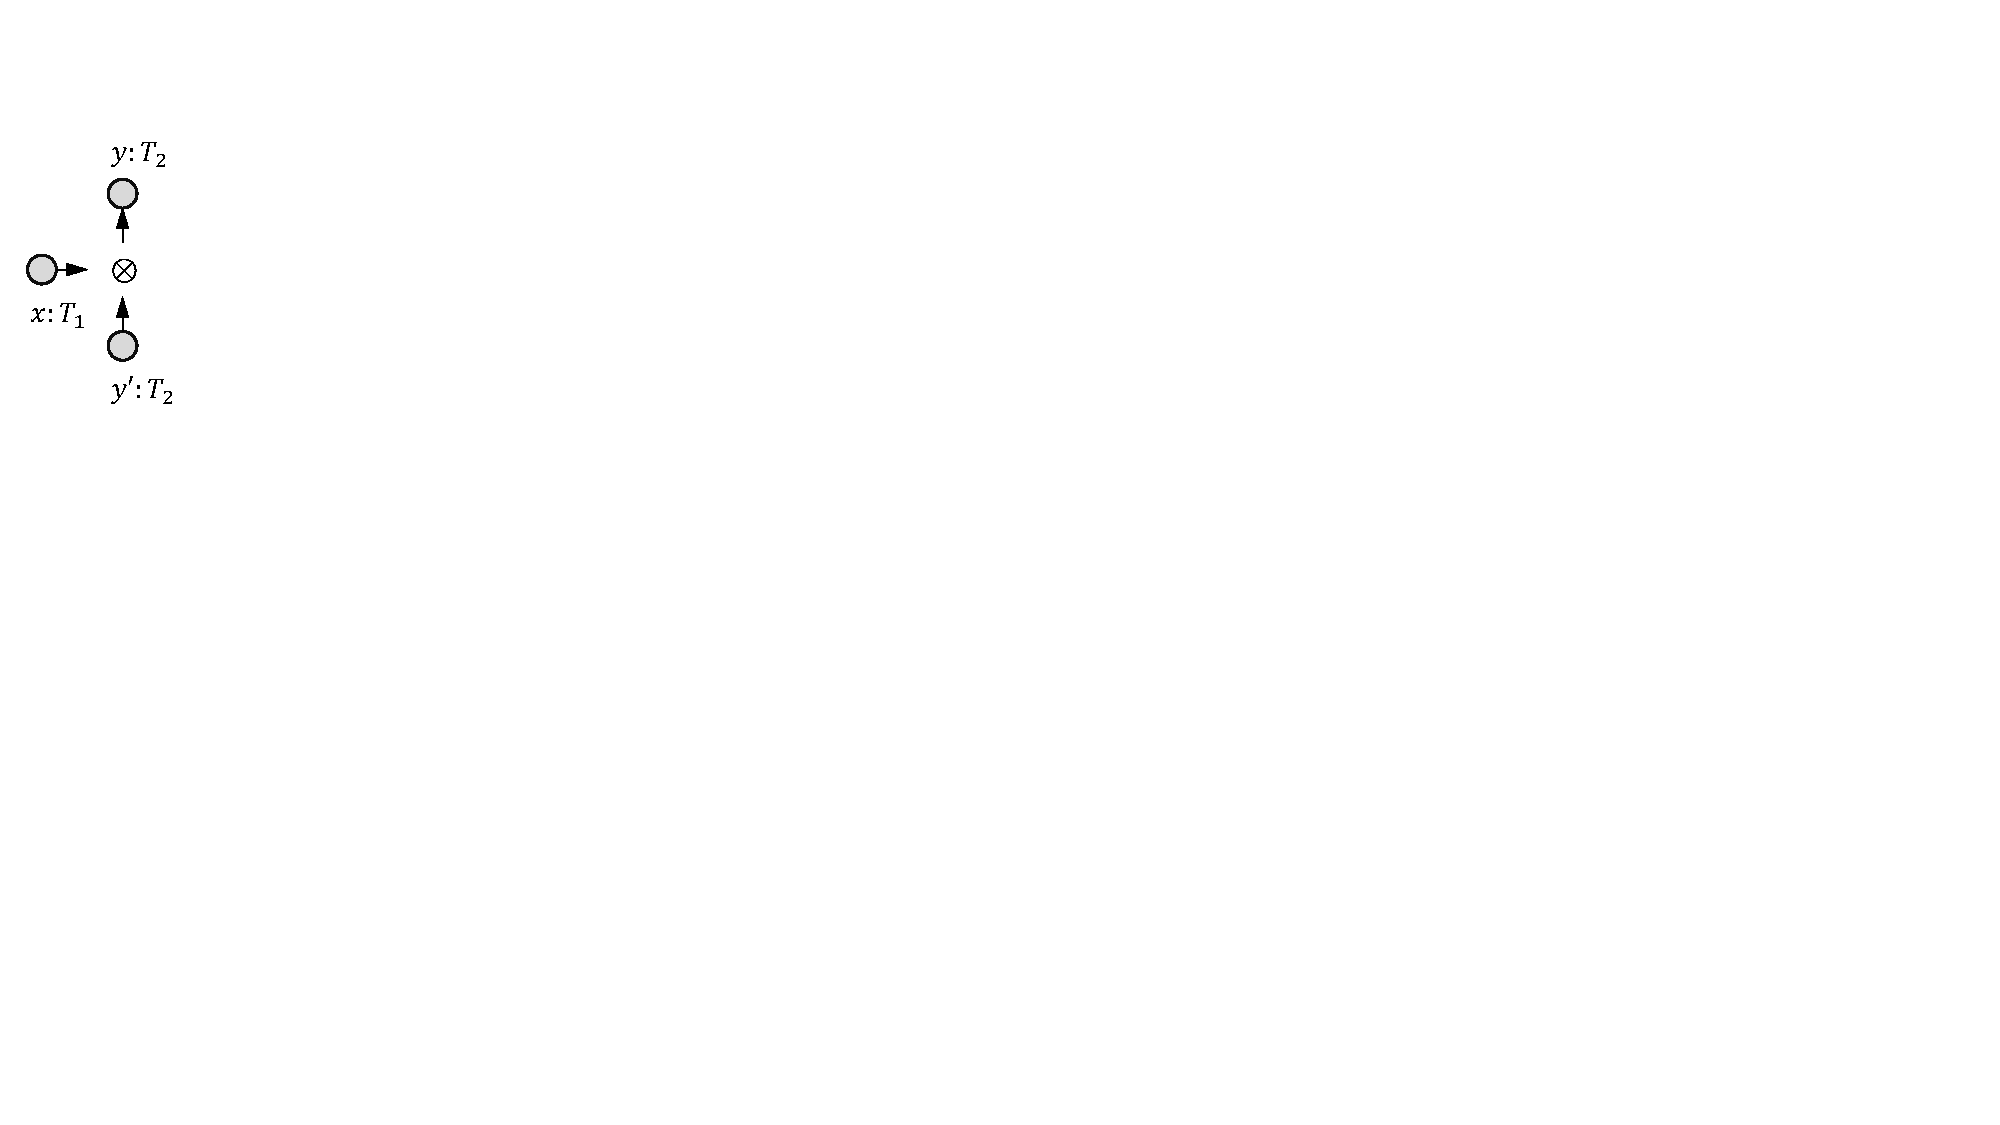
\includegraphics[width=0.1\textwidth]{figures/scan_step.pdf}
%     \caption{A single RNN computation step.}
%     \label{scan-step}
% \end{figure}

% Figure \ref{rnn-layer1} shows an algorithm developer's conceptual model of an RNN layer (the unrolled computational graph in mainstream deep learning frameworks) applied to tokens from a sequence.

% \begin{figure}[h]
%   \centering
%   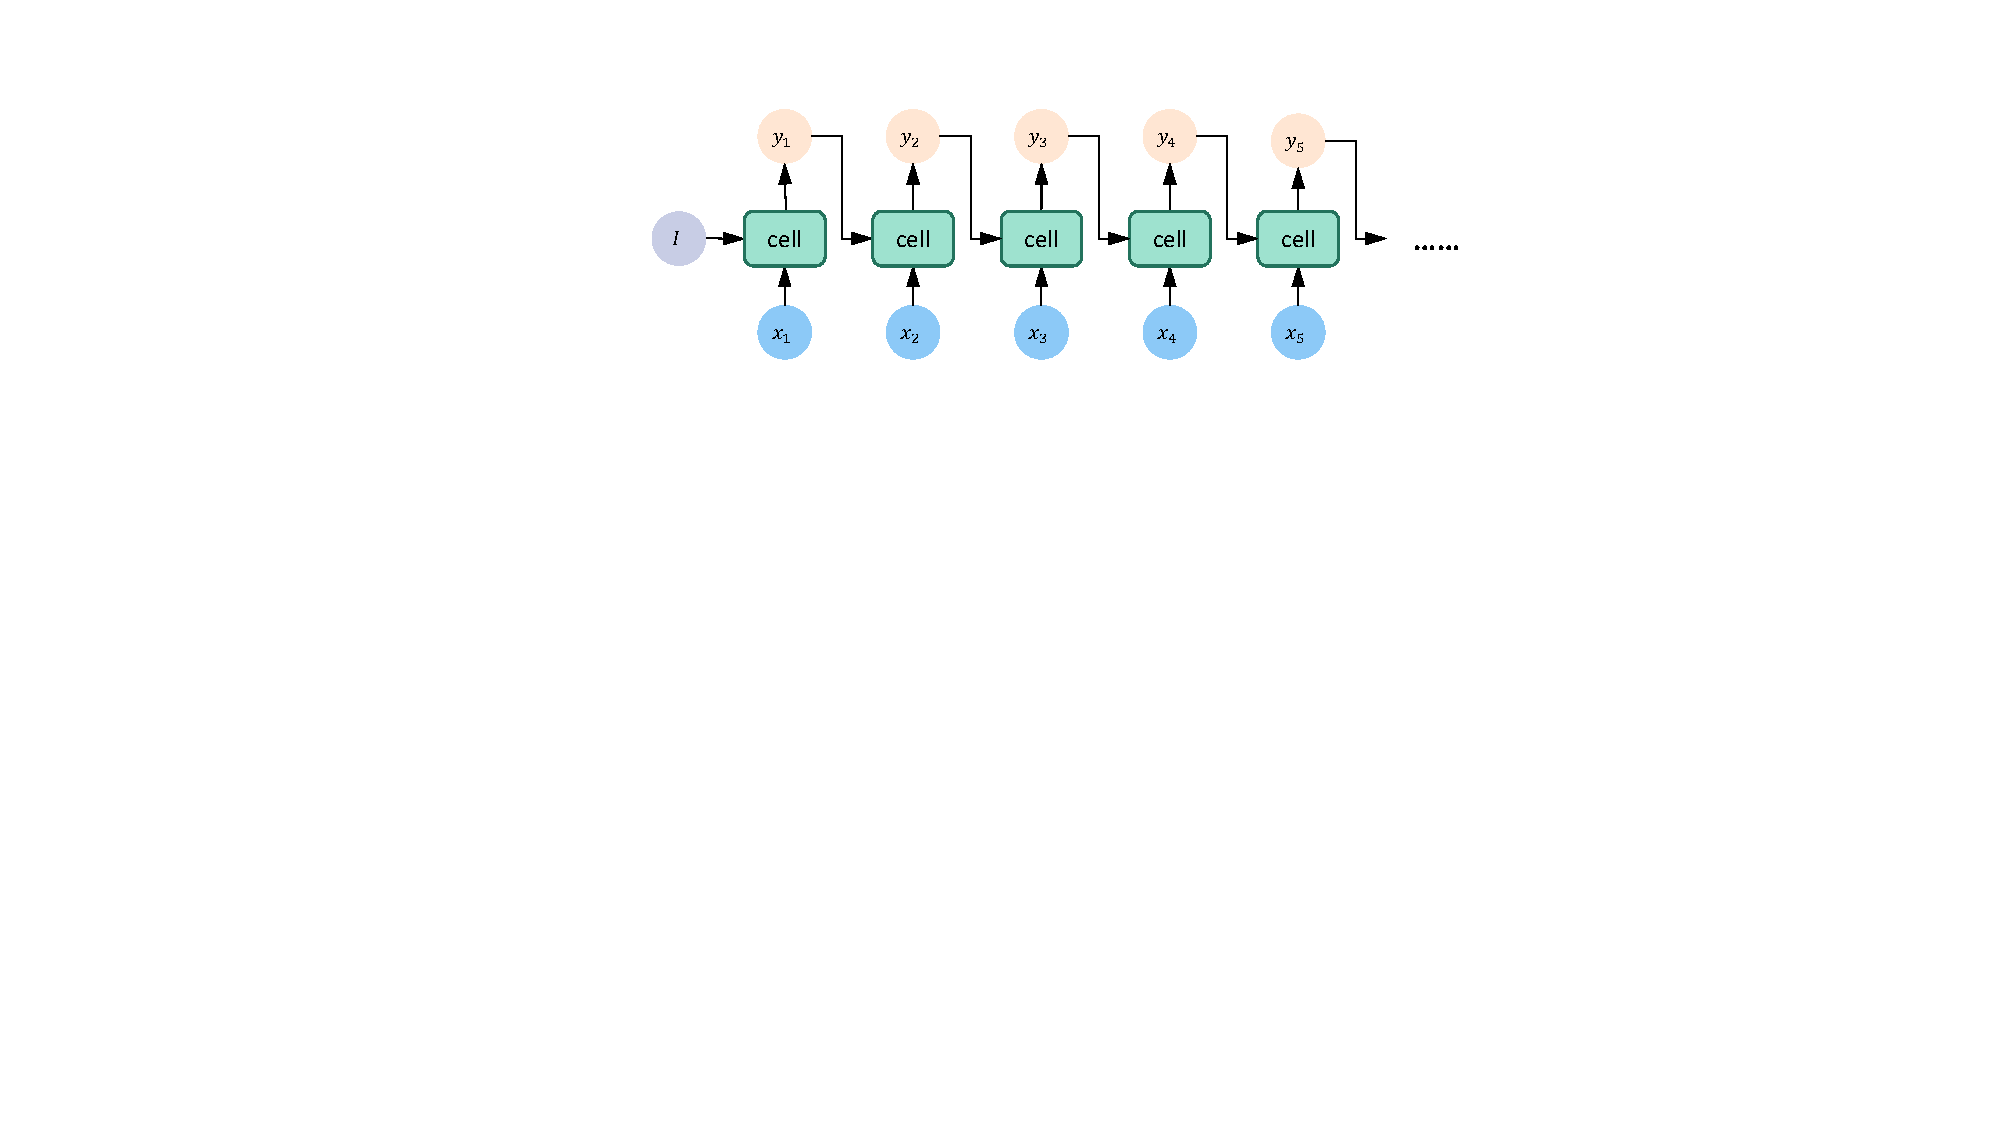
\includegraphics[width=0.5\textwidth]{figures/rnn_layer1.pdf}
%   \caption{An algorithm developer's conceptual model of an RNN layer applied to a single sequence.}
%   \label{rnn-layer1}
% \end{figure}

% An RNN layer is usually trained with a batch of sequences. Figure \ref{rnn-layer2} shows applies an RNN layer to multiple sequences simultaneously and Listing \ref{rnn-layer-code} is the corresponding codes using FractalTensor constructs.

% \begin{figure}[h]
%   \centering
%   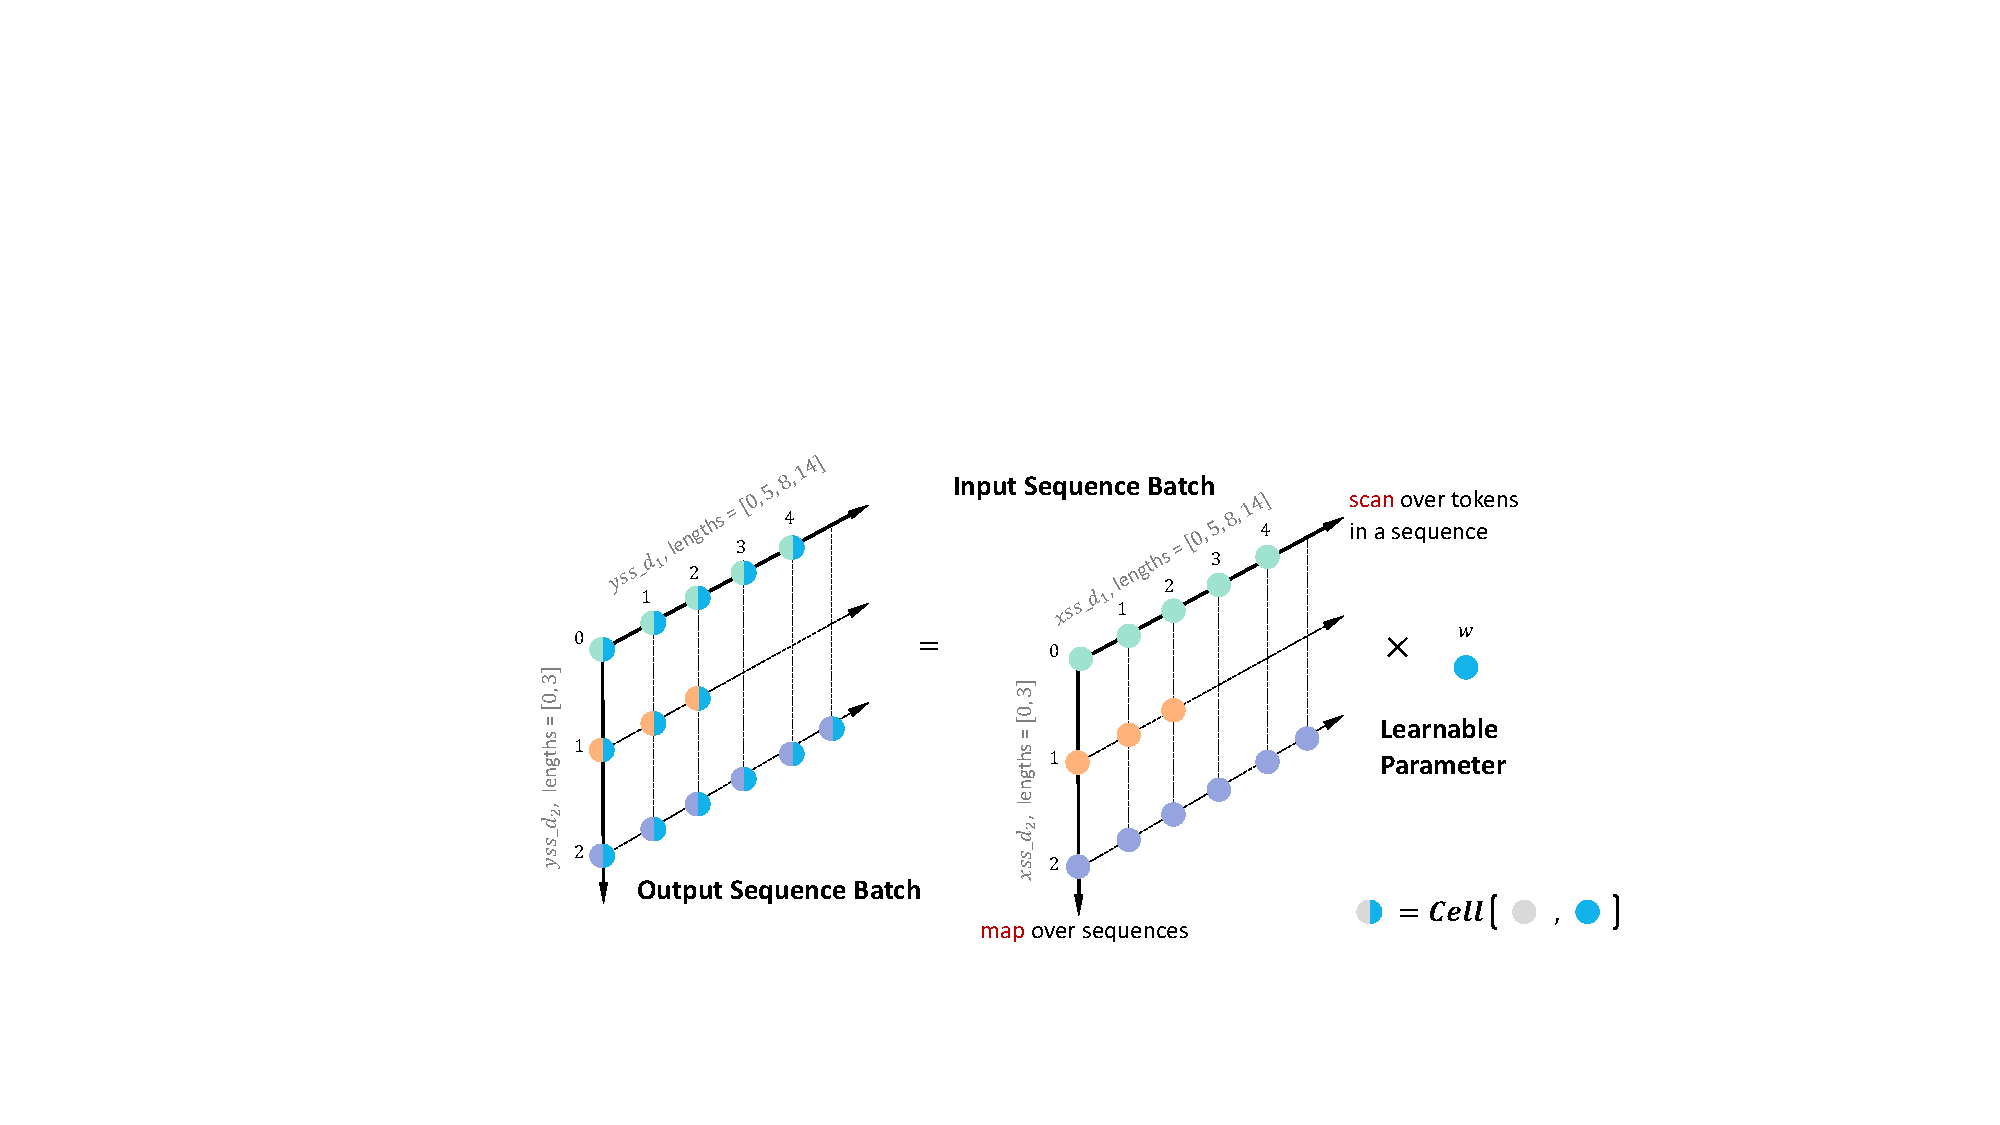
\includegraphics[width=0.6\textwidth]{figures/rnn_layer2.pdf}
%   \caption{An RNN layer applied to multiple sequences.}
%   \label{rnn-layer2}
% \end{figure}

% \lstset{
%   frame=lrtb,
%   backgroundcolor=\color{aliceblue},
%   numbers=left,
%   numbersep=5pt,
%   numbersep=1em,
%   xleftmargin=1em
% }
% \begin{lstlisting}[language=fractaltensor-hello-world, caption={用Parallel Pattern \textcolor{red}{\textit{map}}和\textcolor{red}{\textit{scan}}的嵌套compose 一个RNN layer}, label={rnn-layer-code}]
% xss: [][]float32[1, 512] = ...  // A batch of input sequences
% (:\textbf{\textcolor{dkgreen}{w}}:): float32[512, 512] = ...  // Learnable parameter for the UDF

% // yss: [][]float32[1, 512], the output buffer
% (:\textbf{\textcolor{dkgreen}{yss}}:) = xss.map(xs (:$\Rightarrow$:) {
%     ys = xs.scan(s, x (:$\Rightarrow$:) {
%         y = x @ (:\textbf{\textcolor{dkgreen}{w}}:) + s  // UDF is small math function
%     }, initializer=zeros),
% })
% \end{lstlisting}

% \begin{lstlisting}[language=cplus, caption={Listing \ref{rnn-layer-code}的imperative style 语法等价形}]
% xss: [][]float32[1, 512] = ...  // token batch
% (:\textbf{\textcolor{dkgreen}{w}}:): float32[512, 512] = ... // UDF的可学习参数
% yss: [][]float32[1, 512] = ... // 输出buffer

% L: const int[3] = [5, 3, 6]
% N: int = len(xss)

% for i = [0, N) {  // 对应了全并行的map
%   for j = [0, L[i]) {  // 对应了携带数据流依赖的scan
%     if j == 0:
%       s = zeros
%     else:
%       s = yss[i][j - 1]
%     x = xss[i][j]
    
%     yss[i][j] = x @ w + s
%   }
% }
% \end{lstlisting}
